%! TEX program = xelatex
\documentclass[cn,hazy,blue,11pt,screen]{elegantnote}
\title{Learn Tex}
\author{熊大钧}
\date{\today}

\usepackage{array}

\begin{document}
  \maketitle
\tableofcontents

\section{排版基础\footnote{测试章节脚注。}}
这是一个测试案例
\begin{enumerate}
  \item ctexfont: 默认选项
  \item founder: 方正字体选项
\end{enumerate}
\begin{itemize}
  \item 这是一个item
\end{itemize}
\begin{description}
  \item[Enumerate] nice 
  \item[hello] world!
\end{description}
\begin{center}
    this is a center sentences
\end{center}
\begin{flushleft}
  this is a flushleft sentences
\end{flushleft}
\begin{flushright}
  this is a flushright sentences
\end{flushright}
\centering
this is a centering sentences

\raggedleft
this is a raggedleft sentences

\raggedright
this is a raggedright sentences
\begin{verbatim}
  #include <vector>
\end{verbatim}
\begin{table}[htbp]
  \centering
  \small
  \caption {函数求导表}
  \begin{tabular}{|l|c|c|}
    \hline
    left & right & right \\ 
    \hline
    par pox with & good & nice \\
    \hline
    L   & C & D \\
    \hline
  \end{tabular}
\end{table}
\begin{figure}[htbp]
  \centering
  \begin{minipage}{20em}
    \centering
    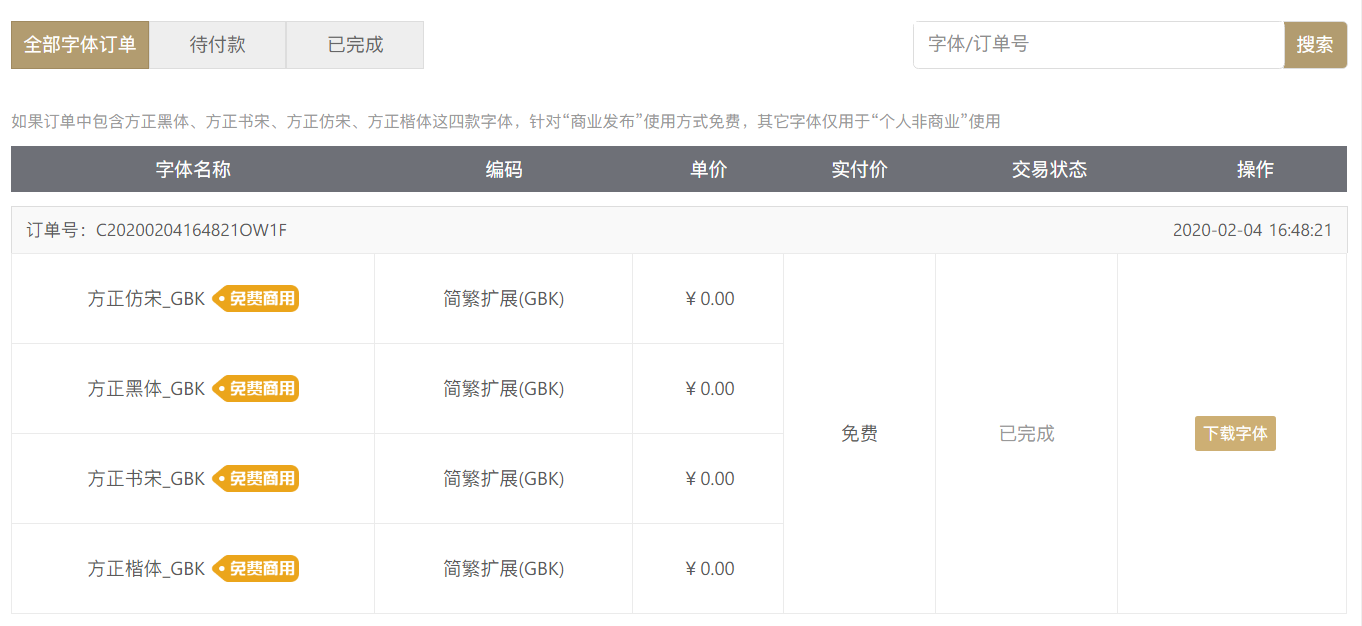
\includegraphics[width=0.4\textwidth]{founder.png}
    \caption{founder}
  \end{minipage}
  \begin{minipage}{20em}
    \centering
    
\includegraphics[width=0.4\textwidth]{wall.jpg}
    \caption{nv}
  \end{minipage}
\end{figure}
\listoffigures
\framebox{Test some words}

\section{Math}
The Py theorem is $a^2 + b^2 = c^2$
The Py theorem is
\begin{equation}
   a^2 + b^2 = c^2\label{1}
\end{equation}
Equation \eqref{1} is called "Gou"
\begin{equation}
   a^2 + b^2 = c^2\tag{yes}
\end{equation}
\[a^2 + b^2 = c^2\]
$a_1, a_2, \dots, a_n$\\
$a_1 + a_2 + \cdots + a_n$\\
In display style:
\[
  3/8 \qquad \frac{3}{8}
  \qquad \tfrac{3}{8}
\]
In text style:
$1\frac{1}{2}$
$1\dfrac{1}{2}$

\colorbox[gray]{0.95}{浅灰色背景}
\href{http://github.com}{Github}
\end{document}
